% Mecánico rotacional: tren de engranajes (tres etapas)
\documentclass[border=5pt]{standalone}
\usepackage{tikz}
\usetikzlibrary{arrows.meta}
\begin{document}
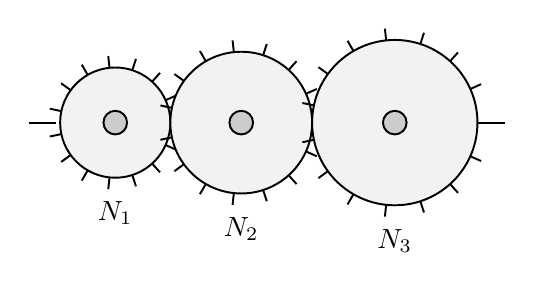
\begin{tikzpicture}[line width=0.7pt]
  \def\gear(#1)(#2)(#3){%
    \foreach \a in {0,24,...,336} \draw ([shift={(#1,0)}]\a:#2) -- ([shift={(#1,0)}]\a:{#2+0.15});
    \draw[fill=black!5] (#1,0) circle (#2);
    \draw[fill=black!20] (#1,0) circle (0.15);
    \node at (#1,{-#2-0.45}) {#3};
  }
  \gear(0)(0.7)($N_1$)
  \gear(1.6)(0.9)($N_2$)
  \gear(3.55)(1.05)($N_3$)
  \draw (-1.1,0) -- (-0.75,0);
  \draw (4.6,0) -- (4.95,0);
\end{tikzpicture}
\end{document}
